%+----------------------------------------------------------------------------+
%| SLIDES: 
%|
%| Contents:	- 60 minutes, 
%| Note: Riprovo a dare il talk dopo che a Wurzburg è andata male.
%|		 Lì ho sbagliato tutti i tempi ma non so stabilire se è stato un problema di scarsa preparazione
%|       , di farmaci, o di stress da brutte notizie sulla crioc.
%|
%|
%|
%| Author: Antonio miti
%| Place: Caprarola, VT
%| Date: 2/3/24
%+----------------------------------------------------------------------------+



%- D0cum3nt ----------------------------------------------------------------------------------------------
\documentclass[10pt,handout]{beamer}



%- Packages -------------------------------------------------------------------------------------------
\usepackage{custom-style}
\usepackage{multicol}
\usepackage{stmaryrd}
\usepackage{animate}
\usetikzlibrary{positioning, arrows}
\usetikzlibrary{shapes}
\usepackage{fontawesome}



%--Beamer Style----------------------------------------------------------------------------------------
\usetheme{toninus}
\setbeamertemplate{section in toc}[sections numbered]



%-- Macros ----------------------------------------------------------------------------------------

\providecommand{\pairing}{\langle\cdot,\cdot\rangle}
\providecommand{\vHam}{\mathscr{v}}
\renewcommand{\checkpoint}[0]{
	\setcounter{tocdepth}{1}
	\addtocounter{framenumber}{-1}
 	\begin{frame}[t]{Outline}
  		%\tableofcontents[currentsection,currentsubsection]
  		%
  		\tableofcontents[currentsection]
		%
		\begin{center}
			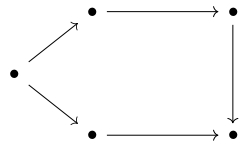
\includegraphics[width=3.5cm]{Pictures/Figure_pentagondiagm_page}
		\end{center}
	\end{frame}
}



%- T1tle P4g3 -------------------------------------------------------------------------------------------
\title{
Multisymplectic observables and higher Courant algebroids
}
\subtitle{\href{https://arxiv.org/abs/2209.05836}{arXiv:2209.05836} (j.w. Marco Zambon)}
\author[AMM]{\href{https://dmf.unicatt.it/miti/}{Antonio Michele Miti}}
\institute[SUR]{
	Sapienza Università di Roma,	Rome, Italy 	\\
	\vspace{.5em}
  \begin{tabular}[h]{ccc}
      \href{https://dipartimenti.unicatt.it/dmf-home?rdeLocaleAttr=it}{
\includegraphics[width=6cm]{./Logos/Sur_logo}} & & 
      \href{https://wis.kuleuven.be/english}{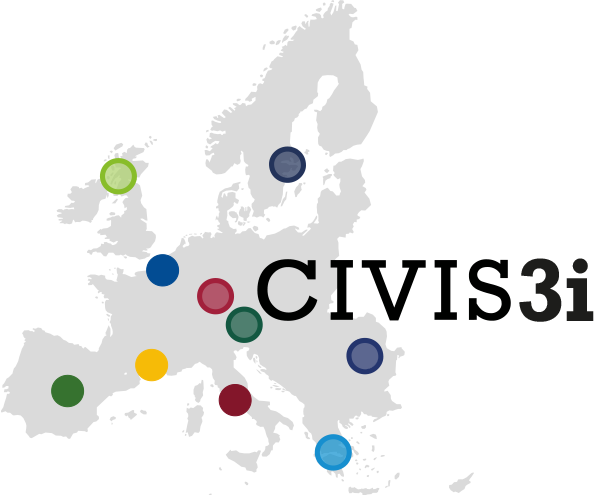
\includegraphics[width=3cm]{Logos/Civis_logo}}
  \end{tabular}    
}

\date[Template_21] % (optional, should be abbreviation of conference name)
{	
	{\vskip 1ex}
	Caprarola,
	\\
	February 2, 2024
}







%---------------------------------------------------------------------------------------------------------------------------------------------------
%- D0cum3nt ----------------------------------------------------------------------------------------------------------------------------------
\begin{document}
%-------------------------------------------------------------------------------------------------------------------------------------------------



\begin{frame}  % Alternative: \maketitle outside of frame
	\titlepage
	\ifHandout
		\tikz[overlay,remember picture]
		{
	    	%	\node at ($(current page.west)+(1.5,0)$) [rotate=90] {\Huge\textcolor{gray}{\today}};
	    	\node[        
	    		draw,
	    		shape border rotate=90,
			isosceles triangle,
			isosceles triangle apex angle=90,
			fill=yellow]
	        		at ($(current page.north east)-(1,1)$) [rotate=-45] {\textcolor{red}{Handout version}};
		}
	\fi
	% European Commission	
		\tikz[overlay,remember picture]
		{
	    	%	\node at ($(current page.west)+(1.5,0)$) [rotate=90] {\Huge\textcolor{gray}{\today}};
	    	\node[        
	    		text width = 3.5cm
			]
	        		at ($(current page.south west)+(1.85,.5)$) [rotate=0] {

					\href{https://dipartimenti.unicatt.it/dmf-home?rdeLocaleAttr=it}{\includegraphics[width=\textwidth]{./Logos/Eu-h2020}}
 		
	        		};
		}
	\end{frame}
	\addtocounter{framenumber}{-1}
\note{
	%\textbf{\underline{OUTLINE}}:
	%\tableofcontents
	\textbf{Abstract:}
	\\
    Until end 2026 (1 year after the end of CIVIS3i)
	All dissemination of results (in any form, including electronic) must:
	(a) display the EU emblem (ie, logo)
	(b) include the text “This project has received funding from the European
		Union’s Horizon 2020 research and innovation programme under grant
		agreement N°101034324.”
    
}
%---------------------------------------------------------------------------------------------------------------------------------------------------




%-------------------------------------------------------------------------------------------------------------------------------------------------
\iffalse \section{Introduction}\fi
%-------------------------------------------------------------------------------------------------------------------------------------------------


%-------------------------------------------------------------------------------------------------------------------------------------------------
\begin{frame}[t] % Hybrid format - Title Page
	%
	\begin{center}
	\color{UniGreen}
		\par\noindent\rule{\textwidth}{0.4pt}\\[.5em]	
		{\bf\Large\emph{Multisymplectic observables }}
		\\
		and 
		{\bf\Large\emph{higher Courant algebroids}}\\
		\par\noindent\rule{\textwidth}{0.4pt}			
	\end{center}
	\vfill

	\centering
	\begin{tikzpicture}
		\node [draw,ellipse callout,UniGreen, minimum height=16em,minimum width=33em,callout relative pointer={(0,1)}] (L1) {};
		\node [text width=28em,text centered] (L2) {
			\textcolor{UniGreen}{\textbf{Honest Goals} of the talk:}
			\\
			\medskip
			\begin{itemize}[<+->]
				\item[•] Recall a certain "gauge-compatibility" condition in \emph{symplectic} geometry 
				   \color{blue}\small (involving $\omega$-twisted Lie alg.oids)
				\item[•] Discuss how this condition extends to \emph{\textbf{multi}symplectic} geometry
				   \color{blue}\small (involving $\omega$-twisted higher Courant alg.oids)
				\item[•] Review certain multisymplectic constructions guided by the above problem.\\
			\end{itemize}
			\medskip
		};
	\end{tikzpicture}

\end{frame}
\addtocounter{framenumber}{-1}
%-------------------------------------------------------------------------------------------------------------------------------------------------


%%-------------------------------------------------------------------------------------------------------------------------------------------------
%\begin{frame}[fragile]{A \emph{pentagonal} diagram in symplectic geometry}
%	Given a \alert{symplectic mfd.} $(M,\omega)$ ...
%	\vfill
%	\begin{center}
%		\includestandalone[width=.95\textwidth]{Pictures/Frame_Embedding_Diagram_symplectic}
%	\end{center}
%	\vspace{3em}
%	\vfill
%	\begin{minipage}[t][8.5em][t]{\textwidth}
%		\begin{itemize}
%			\item<1-> \alert<1>{... there is a naturally associated Poisson algebra ...}
%			\item<2-> \alert<2>{... and also a (standard twisted) Lie Algebroid}.
%			\item<3-> A Lie algebroid is a "controlled" \alert<3>{$\infty$-dimensional Lie algebra.}
%			\item[]<4->
%				\quad\\
%		\vspace{-.75em}
%		\tcbset{colback=white,
%		colbacktitle=white,
%		colframe=red!70!black,
%		boxrule=1pt,
%		colupper=red!70!black,
%		arc=15pt,
%		}
%		\begin{tcolorbox}[enhanced,frame hidden,borderline={0.5pt}{0pt}{blue}]
%			\color{blue}{
%			\textbf{Lemma}: There exists an embedding of Lie Algebras.
%			}
%		\end{tcolorbox}
%		\end{itemize}
%	\end{minipage}
%\end{frame}
%%-------------------------------------------------------------------------------------------------------------------------------------------------

%-------------------------------------------------------------------------------------------------------------------------------------------------
\begin{frame}[fragile]{A \emph{pentagonal} diagram in symplectic geometry}
	Given a \alert{symplectic mfd.} $(M,\omega)$ ...
	\vfill
	\begin{center}
		\includestandalone[width=.95\textwidth]{Pictures/Frame_Embedding_Diagram_symplectic}
	\end{center}
	\vfill
	\begin{minipage}[t][8.5em][t]{\textwidth}
		\only<1-3>{One can naturally associate:}
		\begin{itemize}
			\only<1-3>{
			\item<1-> a \alert<1>{Poisson algebra} w/ $$\{f,g\}_\omega = -\iota_{\vHam_f}\iota_{\vHam_g} \omega$$
			\item<2-> a \alert<2>{(standard twisted) Lie Algebroid};
			\item<3->[-] A Lie algebroid is a "controlled" $\infty$-dimensional Lie algebra w/
			\begin{displaymath}
					\left[\binom{x_1}{f_1},\binom{x_2}{f_2}\right]_\omega
					~=~
					\binom{[x_1,x_2]}{x_1(f_2)-x_2(f_1)-\omega(x_1,x_2)}
				\end{displaymath}
			}
			\item[]<4->
				\quad\\
				\begin{thmblock}[There exists an embedding of Lie algebras.]
					\begin{displaymath}
						\begin{tikzcd}
							\Psi~:&[-1em] (C^{\infty}(M), \{\cdot,\cdot\}_\omega) \ar[r,"\Psi"]& 
							(\Gamma(TM\oplus \mathbb{R}), [\cdot,\cdot]_\omega)
							\\[-2em]
							& f \ar[r,mapsto] & \binom{\mathscr{v}_f}{f}
						\end{tikzcd}		
					\end{displaymath}
				\end{thmblock}
		\end{itemize}
	\end{minipage}
\end{frame}
\note{}
%-------------------------------------------------------------------------------------------------------------------------------------------------


%-------------------------------------------------------------------------------------------------------------------------------------------------
\begin{frame}[fragile]{A \emph{pentagonal} diagram in symplectic geometry}
	%
	Consider two \alert{gauge-related} symplectic mfd. $(M,\omega)$ and $ (M,\widetilde{\omega})$.
	~~ \alert{($\widetilde{\omega} = \omega - \d B$)}
	%
	\begin{center}
			\includestandalone[width=.8\textwidth]{Pictures/hyb-Frame_BigDiagram_symplectic}
	\end{center}
		\vfill
	\begin{minipage}[t][8em][t]{\textwidth}
		\begin{itemize}
			\only<3-4>{
				\item<3-> There is a natural \alert<3>{isomorphism in the Lie Alg.oids category} \emph{($B$-transformation)}
					\begin{displaymath}
						\binom{x}{f} \mapsto \binom{x}{f-\iota_x B} ~.
					\end{displaymath}~.
				\item<4-> It descends to an \alert<4>{isomorphism of Lie algebras}.
			}
			\only<6-8>{
				\item<6-> \vspace{-2em}Consider an infinitesimal \alert<6>{Hamiltonian group action} $\mathfrak{g}\curvearrowright M$ w.r.t. both $\omega$ and $\tilde{\omega}$.
				\item<7-> let be $f:\mathfrak{g} \to C^\infty(M)_\omega$ and $\tilde{f}:\mathfrak{g} \to C^\infty(M)_{\tilde{\omega}}$ two comoment map s.t.
				\begin{displaymath}
					\tilde{f}(\xi) = f(\xi) - \iota_{\underline{\xi}}B
				\end{displaymath}
				}
			\item[]						
		\end{itemize}
	\only<2>{
		\vspace{-.75em}
		\begin{center}
		\tcbox[enhanced,frame hidden,borderline={0.5pt}{0pt}{red,dashed}]{	
			\alert{
			\faQuestionCircle \qquad
				{How can we compare the two \emph{observables} algebras?}
			\qquad \faQuestionCircle		
			}
		}
		\end{center}
	}
	\only<5>{
		\vspace{-.75em}
		\begin{center}
		\tcbox[enhanced,frame hidden,borderline={0.5pt}{0pt}{red,dashed}]{	
			\alert{
			\faQuestionCircle \qquad
				{How can we close the left-hand side?}
			\qquad \faQuestionCircle		
			}
		}
		\end{center}
	}
	\only<8->{
		\vspace{-.75em}
		\tcbset{colback=white,
		colbacktitle=white,
		colframe=red!70!black,
		boxrule=1pt,
		colupper=red!70!black,
		arc=15pt,
		}
		\begin{tcolorbox}[enhanced,frame hidden,borderline={0.5pt}{0pt}{blue}]
			\color{blue}{
			\textbf{Lemma}: The central pentagon commutes!
			}
			\hfill \hyperlink{frame:whyNoVertArrow}{\color{gray}$[>>]$}%\beamerskipbutton{}}
		\end{tcolorbox}
	\vfill
	
	}
	\end{minipage}	
\end{frame}
%-------------------------------------------------------------------------------------------------------------------------------------------------


%%-------------------------------------------------------------------------------------------------------------------------------------------------
%\begin{frame}[fragile]{Compatibility between gauge transformations and comoment maps}
%	%
%	Consider $(M,\omega)$ \alert{symplectic mfd.}
%	%
%	\begin{center}
%			\includestandalone[width=.8\textwidth]{Pictures/Frame_BigDiagram_symplectic}
%	\end{center}
%	%
%	\vspace{-1em}
%	\vfill
%	\begin{minipage}[t][8em][t]{\textwidth}
%		\begin{itemize}
%			\only<2>{
%				\item<2-> Consider a second gauge-related symplectic structure on $M$
%					\begin{displaymath}
%						\tilde{\omega} = \omega + d B \qquad \text{with} \quad B\in \Omega^1(M).
%					\end{displaymath}
%			}
%			\only<3-4>{
%				\item<3-> There is a natural isomorphism in the Lie Alg.oids category \emph{($B$-transformation)}
%					\begin{displaymath}
%						\binom{x}{f} \mapsto \binom{x}{f-\iota_x B} ~.
%					\end{displaymath}
%			}
%			\only<6-7>{
%				\item<6-> Consider an infinitesimal group action $\mathfrak{g}\circlearrowleft M$ which is Hamiltonian w.r.t. both $\omega$ and $\tilde{\omega}$.
%				\item<7-> let be $f:\mathfrak{g} \to C^\infty(M)_\omega$ and $\tilde{f}:\mathfrak{g} \to C^\infty(M)_{\tilde{\omega}}$ two comoment map s.t.
%				\begin{displaymath}
%					\tilde{f}(\xi) = f(\xi) - \iota_{\underline{\xi}}B
%				\end{displaymath}
%				}
%			\item[]						
%		\end{itemize}
%	\only<5>{
%		\vspace{-.75em}
%		\begin{center}
%		\tcbox[enhanced,frame hidden,borderline={0.5pt}{0pt}{red,dashed}]{	
%			\alert{
%			\faQuestionCircle \qquad
%				{How can we close the left-hand side?}
%			\qquad \faQuestionCircle		
%			}
%		}
%		\end{center}
%	}
%	\only<8->{
%		\vspace{-.75em}
%		\tcbset{colback=white,
%		colbacktitle=white,
%		colframe=red!70!black,
%		boxrule=1pt,
%		colupper=red!70!black,
%		arc=15pt,
%		}
%		\begin{tcolorbox}[enhanced,frame hidden,borderline={0.5pt}{0pt}{blue}]
%			\color{blue}{
%			Lemma: The central pentagon commutes!
%			}
%		\end{tcolorbox}
%	\vfill
%	}
%	\only<9->{
%		\vspace{-.75em}
%		\begin{center}
%		\tcbox[enhanced,frame hidden,borderline={0.5pt}{0pt}{red,dashed}]{	
%			\alert{
%			\faQuestionCircle \qquad
%				{What happens in the higher (n-plectic) case?}
%			\qquad \faQuestionCircle		
%			}
%		}
%		\end{center}
%	}
%	\end{minipage}	
%\end{frame}
%\note[itemize]{
%	\item The horizontal embedding is  $f \mapsto (v_f,f)$;
%	\item Vertical maps are also known as \emph{Gauge transformations}
%	\item upshot: 
%	\begin{enumerate}
%		\item 
%	\end{enumerate}
%}
%%-------------------------------------------------------------------------------------------------------------------------------------------------

%-------------------------------------------------------------------------------------------------------------------------------------------------
\begin{frame}[fragile]{Why not a direct vertical arrow?}\label{frame:whyNoVertArrow}
	\begin{center}
			\includestandalone[width=.7\textwidth]{Pictures/Frame_BigDiagram_verticalArrow}
	\end{center}
	\vfill
	\begin{itemize}
		\item<2-> Assume exists \alert<2>{$\chi:C^\infty(M)_\omega \to C^\infty(M)_{\widetilde{\omega}}$} ~s.t. the square commutes.
				\begin{displaymath}
					\begin{cases}
						\chi(f) =& f - \iota_{\vHam_f} B
						\\
						\widetilde{\vHam}_{\chi(f)} =& \vHam_f
					\end{cases}
				\end{displaymath}
		\item<3-> Then
			\begin{align*}
				d \chi(f) &= - \iota_{\vHam_f}\omega - d \iota_{\vHam_f} B \\
				\parallel & \\
				-\iota_{\widetilde{\vHam}_{\chi(f)}} \widetilde{\omega} &= -\iota_{\vHam_f} \omega + \iota_{\vHam_f} d B
			\end{align*}
		\item<4-> I.e. $$\mathcal{L}_{\vHam_f} B = 0 ~ \forall f \in C^\infty(M) \qquad \qquad \text{\alert{contradiction!}}$$
	\end{itemize}
	\hfill \hyperlink{frame:pentagonMotivation}{\color{gray}$[<<]$}%\beamerskipbutton{}}
\end{frame}
%-------------------------------------------------------------------------------------------------------------------------------------------------

%-------------------------------------------------------------------------------------------------------------------------------------------------
\begin{frame}[fragile]{A \emph{pentagonal} diagram in symplectic geometry}\label{frame:pentagonMotivation}
	%
	%Consider two \alert{gauge-related} symplectic mfd. $(M,\omega)$ and $ (M,\widetilde{\omega})$.
	We end up with a pentagonal diagram ...
	%
	\begin{center}
			\includestandalone[width=.8\textwidth]{Pictures/hyb-image_BigDiagram_symplectic}
	\end{center}
	%
	\vfill
	\begin{minipage}[t][8em][t]{\textwidth}
	\centering
	\vspace{-2em}
	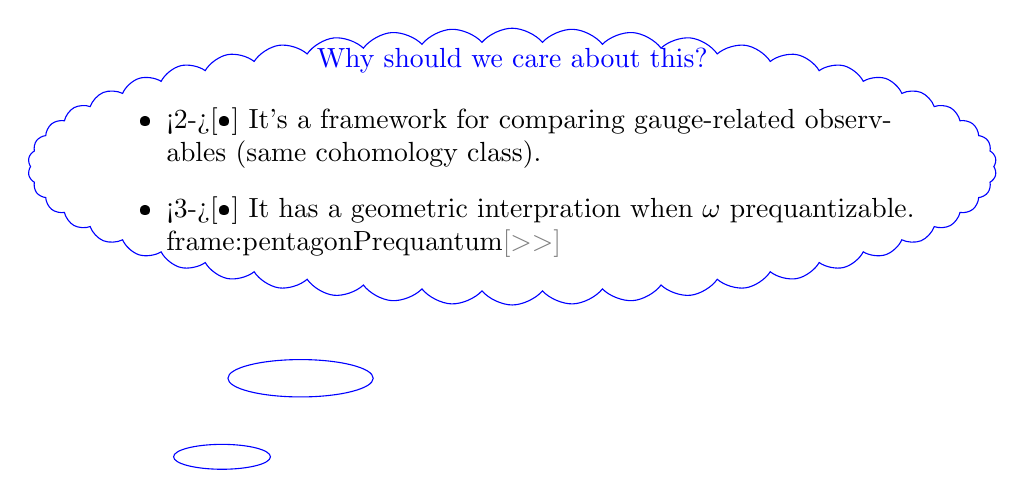
\begin{tikzpicture}
		\node [draw,cloud callout,cloud puffs=50,cloud puff arc=100,blue, minimum height=10em,minimum width=35em,callout relative pointer={(-2,-2)}] (L1) {};
		\node [text width=30em,text centered] (L2) {
			\textcolor{blue}{Why should we care about this?}
			\\
			\begin{itemize}
				\item<2->[•] It's a framework for comparing gauge-related observables (same cohomology class).
				\item<3->[•] It has a geometric interpration when $\omega$ \alert{prequantizable}.
				\hfill \hyperlink{frame:pentagonPrequantum}{\color{gray}$[>>]$}%\beamerskipbutton{}}
			\end{itemize}
			\medskip
		};
	\end{tikzpicture}
	\end{minipage}	
		
\end{frame}
%-------------------------------------------------------------------------------------------------------------------------------------------------

%-------------------------------------------------------------------------------------------------------------------------------------------------
\begin{frame}[fragile]{Pentagonal diagram in the \emph{prequantizable} case}\label{frame:pentagonPrequantum}
	Assume $\omega$ is \alert{prequantizable}:
	\pause
	%
		\begin{columns}
			\begin{column}{.6\linewidth}
				\begin{itemize}
					\item<2-> $\pi:P\to M$ \small associated $S^1$ bundle;
					\item<3-> $E\in \mathfrak{X}(P)$ \small fundamental v.f. of $S^1\curvearrowright P$;
					\item<4-> $\theta\in \Omega^1(P)^{S^1}$ \small connection $1$-form  s.t. $d \theta = \pi^\ast \omega$.
				\end{itemize}
			\end{column}
			\begin{column}{.4\linewidth}
				\begin{center}
					\includestandalone[width=1\textwidth]{Pictures/Frame_prequantum}
				\end{center}	
			\end{column}
		\end{columns}
	\pause \pause \vfill
	The Lie algebra map
	\begin{displaymath}
		\big(C^\infty(M),\{\cdot,\cdot\}_\omega\big) \xrightarrow{\Psi_\omega} 
		\big(\Gamma(TM\oplus\mathbb{R}),[\cdot,\cdot]_\omega\big)
	\end{displaymath}
	%
	\vfill
	factors through the Lie algebra of \emph{\alert{infinitesimal quanto-morphisms}}
	%
	\pause
	\begin{displaymath}
		Q(P,\theta)= \left \lbrace 
			Y \in \mathfrak{X}(P) 
			~ \Big\vert ~
			\mathcal{L}_Y \theta = 0
			\right \rbrace~.
	\end{displaymath}		
	
	
	\hfill \hyperlink{frame:scopeTalk}{\color{gray}$[<<]$}%\beamerskipbutton{}}
\end{frame}
%-------------------------------------------------------------------------------------------------------------------------------------------------



%-------------------------------------------------------------------------------------------------------------------------------------------------
\begin{frame}[fragile]{Pentagonal diagram in the \emph{prequantizable} case \hfill (cont.)}
	\begin{center}
			\includestandalone[width=.8\textwidth]{Pictures/Frame_prequantumDiagram}
	\end{center}	
	\vfill
	\begin{enumerate}
		\item<2-> Start from the prequantization map (isomorphism)
					$$\textrm{Preq}_\theta: f \mapsto \vHam_f^{Hor \theta} + (\pi^\ast f ) E $$
					\hfill {\tiny ( where $Hor \theta$ is the horizontal lift);}
		\item<3-> Observe that $Q(P,\theta) \subset \mathfrak{X}^{S^1}$;
		\item<4-> By definition, $\mathfrak{X}^{S^1}= \Gamma(\textrm{at}(P))$ where $\textrm{at}(P)$ is the Atiyah Lie algebroid associated to the principal bundle $P\to M$.
		\item<5-> $\textrm{at}(P)$ is defined by the s.e.s. $0\to \mathbb{R} \to \textrm{at}(P) \to TM \to 0$,
		\\ $\theta$ provides a splitting, i.e. an isomorphism
		\begin{displaymath}
			\morphism{\sigma_\theta}{TM\oplus \mathbb{R}}{\textrm{at}(P)}
			{\binom{v}{c}}{v^{Hor \theta} + c \cdot E}~.
		\end{displaymath}
	\end{enumerate}
	
	\hfill \hyperlink{frame:scopeTalk}{\color{gray}$[<<]$}%\beamerskipbutton{}}
\end{frame}
%-------------------------------------------------------------------------------------------------------------------------------------------------



%-------------------------------------------------------------------------------------------------------------------------------------------------
\begin{frame}[t]{Scope of the talk}\label{frame:scopeTalk}
		\begin{center}
		\tcbox[enhanced,frame hidden,borderline={0.5pt}{0pt}{red,dashed}]{	
			\alert{
			\faQuestionCircle \qquad
				{\bf  What happens in the (higher) $n$-plectic case?}
			\qquad \faQuestionCircle		
			}
		}
		\end{center}
		\vfill

	\only<2->{
		{
			\color{UniGreen}
			\par\noindent\rule{\textwidth}{0.4pt}	
			\\ {\bf  Outline of the talk:} \\[-.5em]
			\par\noindent\rule{\textwidth}{0.4pt}			
		}
		\vspace{-1.5em}
		\setcounter{tocdepth}{1}
		\tableofcontents
	}
\end{frame}
%-------------------------------------------------------------------------------------------------------------------------------------------------







%-------------------------------------------------------------------------------------------------------------------------------------------------
\section{What is \textbf{multisymplectic geometry}?}
\checkpoint	
%-------------------------------------------------------------------------------------------------------------------------------------------------


\begin{frame}[t, fragile]{Multisymplectic manifolds} %Fragile -->workaround tikzcd
	\begin{center}
		$-$ \emph{multisymplectic means \textbf{going higher} in the degree of $\omega$} $-$
	\end{center}
	\pause
	\begin{defblock}[$n$-plectic manifold ~\emph{(Cantrijn, Ibort, De Le\'on)} \cite{Cantrun2017}]
		\includestandalone[width=0.95\textwidth]{Pictures/Figure_multisym}	
	\end{defblock}
	%
	\pause
	%
	\begin{defblock}[Non-degenerate $(n+1)$-form]
		\begin{columns}
			\begin{column}{.45\linewidth}
				\centering{
				The $\omega^\flat$ (flat) bundle map is injective.
				}
			\end{column}
			\begin{column}{.5\linewidth}
						\vspace{-.5em}
				\[
				\begin{tikzcd}[column sep= small,row sep=0ex,
				/tikz/column 1/.append style={anchor=base east}]
				    \omega^\flat \colon T M \ar[r]& \Lambda^n T^\ast M \\
  						 (x,u) \ar[r, mapsto]& (x,\iota_{u} \omega_x)						
				\end{tikzcd}	
				\]
			\end{column}
		\end{columns}
	\end{defblock}		
	\vfill
	%
	%
	\pause
	\begin{block}{Examples:}
		\begin{itemize}
			\item[$\bullet$] 1-plectic $=$ symplectic
			\item[$\bullet$] Any oriented $(n+1)$-dimensional manifold is $n$-plectic w.r.t. the volume form.
			\item[$\bullet$] The multicotangent bundle $\Lambda^n T^\ast Q$ is naturally $n$-plectic.
		\end{itemize}
	\end{block}			 
%

\end{frame}

\begin{frame}[fragile]{Multisymplectic manifolds - mechanics perspective} %Fragile -->workaround tikzcd
	\label{frame:hystMS}
	\begin{block}{Historical motivation}
		Mechanics: geometrical foundations of \textit{(first-order)} field theories.
		\begin{itemize}
		 \item[•] Kijowski, W. Tulczyjew \cite{Kijowski1979}; %(1979)
		 \item[•] Cariñena, Crampin, Ibort \cite{Carinena1991b};% (1991)
		 \item[•] Gotay, Isenberg, Marsden, Montgomery \cite{Gimmsy1};%(1998)
		 \\ $\cdots$
		\end{itemize}
	\end{block}
	%
	\pause
	\begin{table}
		\ifHandout
		%
		\else
		\only<2>{
		\begin{tabular}{|p{0.2\textwidth}|p{0.3\textwidth}|p{0.35\textwidth}|} 
            \hline
            \parbox[][20pt][c]{0.2\textwidth}{mechanics} & \multicolumn{2}{c|}{geometry} \\
            \hline
            \parbox[][20pt][c]{0.2\textwidth}{phase space} & symplectic manifold &  \\[.25em]
            \parbox[][20pt][c]{0.2\textwidth}{classical \\ observables} & Poisson algebra &  \\[.25em]
            \parbox[][20pt][c]{0.2\textwidth}{symmetries} &  group actions admitting comoment map &  
            \\
            \hline
  \multicolumn{1}{c}{}
            &  \multicolumn{1}{@{}c@{}}{$\underbrace{\hspace*{.3\textwidth}}_{\text{point-like particles systems}}$} 
            &  \multicolumn{1}{@{}c@{}}{}              \\
		\end{tabular}
		}
		\fi
		\onslide<3->{
		\begin{tabular}{|p{0.2\textwidth}|p{0.3\textwidth}|p{0.35\textwidth}|} 
            \hline
            \parbox[][20pt][c]{0.2\textwidth}{mechanics} & \multicolumn{2}{c|}{geometry} \\
            \hline
            \parbox[][20pt][c]{0.2\textwidth}{phase space} & symplectic manifold & multisymplectic manifold \\[.25em]
            \parbox[][20pt][c]{0.2\textwidth}{classical \\ observables} & Poisson algebra & $L_\infty$-algebra \\[.25em]
            \parbox[][20pt][c]{0.2\textwidth}{symmetries} &  group actions admitting comoment map & group actions admitting (homotopy) comomentum map
            \\
            \hline
  			\multicolumn{1}{c}{}
            &  \multicolumn{1}{@{}c@{}}{$\underbrace{\hspace*{.3\textwidth}}_{\text{point-like particles systems}}$} 
            &
            \multicolumn{1}{@{}c@{}}{$\underbrace{\hspace*{.3\textwidth}}_{\text{field-theoretic systems}}$} 
               \\
		\end{tabular}
		}
	\end{table}		 
 	\hfill \hyperlink{frame:GIMMSY_construction}{\color{gray}$[>>]$}%\beamerskipbutton{}}
 
	
%
\end{frame}
\note[itemize]{
	\item Multisymplectic ($n$-plectic) geometry is a generalization of symplectic geometry where a closed, non degenerate $n+1$-form $(n\geq 1)$  takes the place of the symplectic 2-form
	
	\item multisymplectic means \emph{going higher} in the degree of $\omega$
	
	\item non degeneracy means $\iota_v\omega = 0 \Leftrightarrow v=0$.
	
	\item examples: 
	\\1-plectic $=$ symplectic, 
	\\any oriented $(n+1)$-dimensional manifold is $n$-plectic w.r.t. the volume form
	\\the multicotangent bundle $\Lambda^n T^\ast Q$ is naturally $n$-plectic (see frame extra-\ref{Frame:Ms-Field-Mechanics})
	
	\item Observe also that, by degree reason, when $n$ is equal to $1$ or $dim(M)+1$ an injective flat map $\flat$ is also bijective.
	
	\item It is important to stress that mechanical systems are not the only source instances of this class of of structures. 
				e.g. any semisimple Lie groups has associated a 2-plectic structure and any oriented $n+1$ dimensional manifold is naturally $n$-plectic.
				

}
%---------------------------------------------------------------------------------------------------------------------------------------------------




%-------------------------------------------------------------------------------------------------------------------------------------------------
\begin{frame}[fragile]{A multisymplectic manifold in Lagrangian Field Theory}\label{frame:GIMMSY_construction}
	\begin{center}
		\includestandalone[width=.5\textwidth]{Pictures/Frame_GIMMSY}
	\end{center}	
	\vfill
	
	Consider a \emph{\bf{first-order Lagrangian Field Theory}}:
	\begin{itemize}
		\item<1-> {\color{blue} Kinematics} is encoded by a {\color{blue} \emph{configuration bundle}};
		\item<2-> {\color{red} Dynamics} is encoded by a {\color{red} \emph{Lagrangian density}};
		\item<3-> The {\color{orange} multicontangent bundle} is naturally $n$-plectic with $\omega := d \theta$ and \\
		$\theta \in \Omega^n(\Lambda)$ the tautological $n$-form
		{\small
		\begin{displaymath}
			\left[ \iota_{u_1 \wedge \ldots \wedge u_n} \theta \right]_\eta 
			= \iota_{u_1 \wedge \ldots \wedge u_n} \pi^\ast \eta 
			\qquad \qquad \forall \eta \in \wedge^n T^* E \, , \: \forall u_i \in T_\eta (\wedge^n T^* E) 		
		\end{displaymath}
		}
		\item<4-> The multisymplectic $(n+1)$-form is pulled back to $J^1 E$ through the \emph{Legendre transformation} $\mathbb{F}\Lag: J^1 E \to (J^1 E)^\ostar$
    given intrinsically by
    {\small
		\begin{displaymath}
        		\Big\langle \mathbb{F}\mathcal{L}(\gamma),\gamma'\Big\rangle=
        		\mathcal{L}\Big(\gamma\Big) + \frac{ d}{ d \epsilon}\mathcal{L}\Big(\gamma +\epsilon(\gamma'-\gamma)\Big)\Bigg\vert_{\epsilon=0} \qquad \forall \gamma,\gamma' \in J^1 E
    		\end{displaymath}
    }

    %
	\end{itemize}
	%
	\vfill
	\hfill \hyperlink{frame:hystMS}{\color{gray}$[<<]$}%\beamerskipbutton{}}
\end{frame}
%-------------------------------------------------------------------------------------------------------------------------------------------------


%-------------------------------------------------------------------------------------------------------------------------------------------------
\section{What is the \textbf{higher analogue} of the \textbf{Poisson algebra}?}
\checkpoint
%-------------------------------------------------------------------------------------------------------------------------------------------------


\begin{frame}{Hamiltonian forms}
	\begin{defblock}[Hamiltonian $(n-1)$-forms]
		\begin{displaymath}
			\Omega^{n-1}_{ham}(M,\omega) 	:=
			\biggr\{ \sigma \in  \Omega^{n-1}(M) \; \biggr\vert \; 
				\exists \vHam_\sigma \in \mathfrak{X}(M) ~:~ 
				\tikz[baseline,remember picture]{\node[rounded corners,
                        fill=orange!5,draw=orange!30,anchor=base]            
            			(target) {$d \sigma = -\iota_{\vHam_\sigma} \omega$ };
            	}				
				~\biggr\} 
			\end{displaymath}
	\end{defblock}
	\pause
	%

	%
	\onslide<2>{
		\tikz[overlay,remember picture]
		{
			\node[rounded corners,
                 fill=orange!5,draw=orange!30,anchor=base]
            	 (base) at ($(current page.north east)-(2,1)$) [rotate=-0,text width=3.5cm,align=center] {\footnotesize{\textcolor{red}{Hamilton-DeDonder-Weyl \\equation}}};
		}	
		\begin{tikzpicture}[overlay,remember picture]
		    	\path[->] (base.south east) edge[bend left,red](target.east);
	    \end{tikzpicture}
	}
	%
	\vspace{-1em}
	\begin{columns}[T]
		\setlength{\belowdisplayskip}{5pt}
		\begin{column}{.50\linewidth}
			%
			\centering \it
			$-$ symplectic case $-$
			\onslide<3->{
			\begin{thmblock}[Observables Poisson algebra]
				$C^\infty(M,\omega)$ endowed with
				\vspace{-.5em}
				\begin{displaymath}
					\lbrace \sigma_1, \sigma_2 \rbrace =			
					~ - \iota_{\vHam_1}\iota_{\vHam_2} \omega 
					~= \mathcal{L}_{\vHam_1} \sigma_2
				\end{displaymath}			
				forms a Poisson algebra.
			\end{thmblock}
			}
			%
			\onslide<4->{
			\vspace{1em}
			\begin{itemize}
				\item[\cmark] Skew-symmetric;
				\item[\cmark] multiplication of observables;
				\item[\cmark] Leibniz Rule;
				\item[\cmark] Jacobi equation;
			\end{itemize}		
			}		
		\end{column}	
		%
		\onslide<1->{\vrule{}}
		%
		\begin{column}{.50\linewidth}
			\centering \it
			$-$ $n$-plectic case $-$
			\onslide<5->{			
			\begin{thmblock}[Observables $L_\infty$-algebra]
				$\Omega^{n-1}_{ham}(M,\omega)$ endowed with
				\vspace{-.5em}
				\begin{displaymath}
					\lbrace \sigma_1, \sigma_2 \rbrace =			
					~ - \iota_{\vHam_1}\iota_{\vHam_2} \omega 
				\end{displaymath}			
				can be extended to a \\ $L_\infty-algebra$.
			\end{thmblock}
			}
			%
			\onslide<6->{
			\begin{itemize}
				\item[\cmark] Skew-symmetric;
				\item[\xmark] multiplication of observables;
				\item[\xmark] Jacobi equation;
				%\\ \hspace*{4.25em} full-fledged Jacobi equation;
				\item[\smark] Jacobi equation \emph{up to homotopies}.
			\end{itemize}			
			}
		\end{column}	
	\end{columns}
\end{frame}
%-------------------------------------------------------------------------------------------------------------------------------------------------

%------------------------------------------------------------------------------------------------
\begin{frame}{Reminder: $L_\infty$ Algebras}

		\emph{
			$L_\infty$-algebra is the notion that one obtains from a Lie algebra when one requires the Jacobi identity to be satisfied only up to a higher coherent chain homotopy.
		}
		\\
		\vspace{.5em}
		\begin{defblock}[$L_\infty$-algebra ~\emph{(Lada, Markl)} ~\cite{Lada1995}]
			\includestandalone{Pictures/Figure_Linfinitydef}
		\end{defblock}	
		%
		%
	\pause
%	\vfill
%	\begin{thmblock}[Rogers \cite{Rogers2010}]
%		The \emph{higher observable algebra} $L_{\infty}(M,\omega)$ 	forms an honest $L_\infty$ algebra.
%		\footnotetext{ Take $\mu_1 = \text{d}$, $\mu_k=\lbrace\dots\rbrace_k$, $L$ is a shifted truncation of the de Rham complex.}
%	\end{thmblock}

	\begin{itemize}
		\item<2-> You can construct a coalgebra out of $L$ 
			{\small \color{UniGreen} (the reduced cofree coalgebra $S^{\geq 1}(L[1]),\Delta)$)}.
		\item<3-> You can assemble all $\mu_k$ to get a coderivation $Q_\mu$
				{\small \color{UniGreen} (the unique lift to a coderivation of the decalage of $ \mu=	\mu_1+\mu_2 + \dots$ }.
		\item<4-> Higher Jacobi is tantamount to having $Q_\mu ^2 = 0$.

	\end{itemize}
\end{frame}
\note[itemize]{
	\item $L_\infty$-algebra is the notion obtained from a Lie algebra requiring that the Jacobi identity is satisfied only up to a higher coherent chain homotopy.
	\item The Lie-n algebra mentioned before is a $L_\infty$ algebra with underlying graded vector space concentrated in degrees $0,1...n$.
	
	\item Definition. We say that a permutation $\sigma \in S_n$ is a $(j,n-j)$-unshuffle, $0\leq j \le1 n$  if $\sigma(1)< \dots < \sigma(j)$ and $\sigma(j+1)<\dots<\sigma(n)$.
	\\
	You can also say that $\sigma$ is a $(j,n-j)$-unshuffle if $\sigma(i)< \sigma(i+1)$ when $i\neq j$.

	\item 	Alternatively, the Jacobiators can be also denoted as $$\displaystyle J_m=\sum_{i+j=m+1} 	\mu_i \triangleleft \mu_j = 0$$
	employing the so-called \emph{ Richardson-Nijenhuis product}
		 $$\mu_i\circ \mu_j := (-)^{i(j+1)}\frac{1}{j!(i-1)!}\mu_i \triangleleft \mu_j\otimes \mathbb{1}_{i-1} \circ \mathcal{A}~,$$
		 where $\mathcal{A}$ denotes the (graded) total skew-symmetrizator.
		 
	\item see frame extra-\ref{Frame:unwapping-Jacobi} for a slightly demystification of the higher Jacobi equations.

	\item more precisely this statement is a proposition/definition

}
%------------------------------------------------------------------------------------------------


%-------------------------------------------------------------------------------------------------------------------------------------------------
\begin{frame}[fragile]{Lie $\infty$-algebra of Observables (higher observables) }
	Let be $(M,\omega)$ a $n$-plectic manifold.
	  	\vfill
	\begin{defblock}[$L_\infty$-algebra of observables ~\emph{(Rogers)} \cite{Rogers2010}]
		\medskip
		\hspace{.25em} Is a cochain-complex $(L,\{\cdot\}_1)$ \\
		\vspace{-1em}
		\begin{center}
			\includestandalone{Pictures/Frame_Observables}
		\end{center}
		\onslide<2->{
			\bigskip
			\hspace{.25em} with $n$ (skew-symmetric) multibrackets $(2 \leq k \leq n+1)$\\
			\vspace{-1em}
			\onslide<3->{
				\begin{center}
					\includestandalone{Pictures/Equation_Multibracket}	
				\end{center}
			}
			\medskip
		}
		%
	\end{defblock}
%	\onslide<3->{
%		\emph{Higher analogue} of the \emph{Poisson algebra structure} associated to a symplectic mfd.
%	\vfill
%	\begin{columns}
%		\hfill
%		\begin{column}{.11\linewidth}	
%			If $n>1$:
%			
%		\end{column}	
%		\begin{column}{.8\linewidth}
%		\begin{itemize}
%			\item[\xmark] \textcolor{red}{we lose} :\quad multiplication of observables, Jacobi equation;
%			%\\ \hspace*{4.25em} full-fledged Jacobi equation;
%			\item[\cmark] \textcolor{green}{we gain} :\quad brackets with arities different than two,\\
%			\hspace*{4.25em}
%			 Jacobi equation \emph{up to homotopies}.
%		\end{itemize}		
%		\end{column}		
%	\end{columns}
%	}
  \end{frame}
%-------------------------------------------------------------------------------------------------------------------------------------------------


%-------------------------------------------------------------------------------------------------------------------------------------------------
\begin{frame}[fragile,shrink]{Multisymplectic Observables - a controversial notion}
	\begin{block}{ Much debate about the "correct" mathematical of \emph{multisymplectic observables}}
		\begin{itemize}
			\item A crucial step for quantization schemes.
			\item Obstructed adoption of this formalism in mechanics.
		\end{itemize}	
	\end{block}		
	%
	\vspace{1.5em} \pause
	\begin{block}{ At least a second competing notion of \emph{multisymplectic observables algebra}}
		\begin{displaymath}
			Leib(M,\omega) = \Big( \Omega_{ham}^{n-1}(M,\omega), \llbracket\cdot,\cdot\rrbracket \Big)
		\end{displaymath}
		with the binary bracket 
		\begin{center}
			\includestandalone{Pictures/Equation_Leibbracket}	
		\end{center}
	\end{block}	
	\vspace{1em} \pause
	\begin{block}{Open Questions:}
		\begin{itemize}
			\item How are the two concepts related?
			\item Do they give what is physically expected to be called an \emph{measurable quantity}?
				\\
				(Folklore conjecture: No, they only give \emph{local observables})				
		\end{itemize}
	\end{block}
\end{frame}
%-------------------------------------------------------------------------------------------------------------------------------------------------


%-------------------------------------------------------------------------------------------------------------------------------------------------
\section{What is the \textbf{higher analogue} of the \textbf{twisted Lie algebroid}?}
\checkpoint	
%-------------------------------------------------------------------------------------------------------------------------------------------------

%-------------------------------------------------------------------------------------------------------------------------------------------------
\begin{frame}[t]{Vinogradov Algebroids}
	\begin{defblock}[Vinogradov algebroid (higher Courant)]
		\includestandalone[width=0.95\textwidth]{Pictures/Frame_vinogradov}		
	\end{defblock}
	\vfill
	\begin{itemize}
		\item<6-> $(n=1) ~ \Rightarrow$ standard twisted \emph{Lie algebroid};
		\item<7-> $(n=2) ~ \Rightarrow$ standard twisted \emph{Courant algebroid};
	\end{itemize}

\end{frame}
%-------------------------------------------------------------------------------------------------------------------------------------------------


%-------------------------------------------------------------------------------------------------------------------------------------------------
\begin{frame}[fragile]{Vinogradov $L_\infty$-algebra}
	Vin. alg.oids 
	$\quad\simeq\quad$ 	
	$NQ$-manifolds {\small($L_\infty$-algebroids)}
	$\quad\Rightarrow\quad$ 
	{\small Associated} $L_\infty$-algebra
	%
	\pause
	\begin{defblock}[Vinogradov $L_\infty$-algebra (Zambon) \cite{Zambon2012}]
		\includestandalone[width=0.95\textwidth]{Pictures/Frame_vinogradov-Linfty}	
	\end{defblock}
	\vfill
	\only<6->{
		\tikz[overlay,remember picture]
		{
			\node[rounded corners,
                 fill=gray!1,draw=gray!30,anchor=base]            
            	 (base) at ($(current page.south)+(0,.5)$) [rotate=-0,text width=10cm,align=center] { \footnotesize{\color{gray}{
            	 $e_i = \binom{X_i}{\alpha_i} \in \mathfrak{X}(M)\oplus \Omega^{n-1}(M)$ 
            	 \quad~,\qquad
            	 $f_i \in \bigoplus_{k=0}^{n-2}\Omega^k(M)$.
            	 }}};
		}			
	}

\end{frame}
%-------------------------------------------------------------------------------------------------------------------------------------------------




%-------------------------------------------------------------------------------------------------------------------------------------------------
\begin{frame}[fragile]{TODO}
	Details sulla ricetta di Zambon per costruire questa Lie infinito algebra.
\end{frame}
%-------------------------------------------------------------------------------------------------------------------------------------------------








%-------------------------------------------------------------------------------------------------------------------------------------------------
\section{What is the \textbf{higher analogue} of the \textbf{comoment map}?}
\checkpoint	
%-------------------------------------------------------------------------------------------------------------------------------------------------

%-------------------------------------------------------------------------------------------------------------------------------------------------
\begin{frame}[t]{Comoment maps}
	Consider a Lie algebra action $v:\mathfrak{g} \to \mathfrak{X}(M)$  preserving the $n$-plectic form $\omega$,
	\vfill

	\vspace{-1em}
	\begin{columns}[T]
		\setlength{\belowdisplayskip}{5pt}
		\begin{column}{.50\linewidth}
			%
			\centering \it
			\onslide<2->{
				$-$ symplectic case $-$
				\begin{defblock}[Comoment map pertaining to $v$]
					Lie algebra morphism
					$$ f: \mathfrak{g} \to C^\infty(M) $$
					such that
					$$ d~f (x) = -\iota_{v_x} \omega \qquad \forall x \in \mathfrak{g}~.$$
				\end{defblock}
			}
		\end{column}	
		%
		\onslide<2->{\vrule{}}
		%
		\begin{column}{.50\linewidth}
			\centering \it
			\onslide<3->{			
				$-$ $n$-plectic case $-$
				\begin{defblock}[Homotopy comoment map \tiny (HCMM)]
					$L_\infty$-morphism 
					$$ (f_k) : \mathfrak{g} \to L_\infty (M,\omega)$$
					such that
					$$ d~f_1(x) = -\iota_{v_x} \omega \qquad \forall x \in \mathfrak{g}~.$$
				\end{defblock}	
			}
		\end{column}	
	\end{columns}	
	%
	\pause
	\vfill
	\centering 
	\onslide<4->{\textbf{-- Conserved quantities --}}
	%
	\vspace{-1em}
	\begin{columns}[T]
		\setlength{\belowdisplayskip}{5pt}
		\begin{column}{.50\linewidth}
			%
			\centering \it
			\onslide<4->{
			\begin{propblock}[Noether Theorem]
				\small Fixed $H\in C^\infty_{\text{Ham}}(M)$ ($\mathfrak{g}$-invariant) ,
				$$\mathcal{L}_{v_H} f(x) = 0 \qquad \forall x \in \mathfrak{g}$$
			\end{propblock}
			}
		\end{column}	
		%
		\onslide<5->{\vrule{}}
		%
		\begin{column}{.50\linewidth}
			\centering \it
			\onslide<5->{			
			\begin{propblock}[RWZ16 Theorem]
				\small Fixed $H\in \Omega^{n-1}_{\text{Ham}}(M)$ ($\mathfrak{g}$-invariant),
				$$\mathcal{L}_{v_H} f_k(p) \in B^k(M) \qquad \forall p \in Z_k(\mathfrak{g})$$			
			\end{propblock}
			}
		\end{column}	
	\end{columns}		
\end{frame}
%-------------------------------------------------------------------------------------------------------------------------------------------------




%-------------------------------------------------------------------------------------------------------------------------------------------------
\begin{frame}{Gauge related multisymplectic manifolds and comoment maps}
	Consider $M$ smooth mfd.
	%
	\begin{defblock}[Gauge related $n$-plectic structures]
		\bigskip
		\begin{columns}[T]
			\setlength{\belowdisplayskip}{5pt}
			\begin{column}{.50\linewidth}
				%
				\centering \it
				$\quad\omega,~ \tilde{\omega}~ \in \Omega^{n+1}(M)$ multisymplectic,
			\end{column}	
			%
			\begin{column}{.50\linewidth}
				\centering \it
				such that $\omega = \tilde{\omega} - d B$
			\end{column}	
		\end{columns}	
		\bigskip	
	\end{defblock}
	%
	\pause
	\vfill
	\par\noindent\rule{\textwidth}{0.4pt}	
	\vfill
	%
	Consider \quad $v:\mathfrak{g} \to \mathfrak{X}(M)$ preserving $\omega$ and $\tilde{\omega}$,
	%\phantom{consider}\quad $\mathcal{L}_{v_\xi}\omega=\mathcal{L}_{v_\xi}\tilde{\omega} = 0 \quad \forall \xi \in \mathfrak{g}$
	\\
	let \qquad$f: \mathfrak{g}\to L_\infty(M,\omega)$ an \emph{homotopy comoment map} ~ w.r.t. $\mathfrak{g}\circlearrowleft (M,\omega)$
	\pause
	\begin{lemblock}[Also $(M,\tilde{\omega})$ admits HCMM $(\tilde{f})$]
		\medskip
		\begin{columns}
			\begin{column}{.325\linewidth}
					\onslide<4->{
						\begin{displaymath}
							\tilde{f}_k = f_k +	
								\tikz[baseline,remember picture]{\node[rounded corners,
	                        		fill=blue!5,draw=blue!30,anchor=base]            
	            					(target) {$\mathrm{b}_k$ };
	            					}	
						\end{displaymath}
					}		
			\end{column}
			\begin{column}{.625\linewidth}	
					\onslide<4->{
						\begin{displaymath}
						%
						\begin{tikzcd}[baseline=(O.base),ampersand replacement=\&]
							|[alias=O]| 
							\tikz[baseline,remember picture]{\node[rounded corners,
	                        		fill=blue!2,draw=blue!30,align=center]            
	            					(base) {$\mathrm{b}_k$};}						
							~:\&[-3em] \Lambda^k\mathfrak{g} \ar[r]\& \Omega^{n-k}(M)
							\\[-2em]
							\& \xi_1\wedge\dots \xi_k \ar[r,mapsto] \&
							(-)^k \iota(v_{\xi_1})\dots \iota(v_{\xi_{x_k}}) B
						\end{tikzcd}		
						\end{displaymath}								
					}		
			\end{column}
		\end{columns}
		\bigskip
		\only<4->{
			\begin{tikzpicture}[overlay,remember picture]
			    	\path[->,opacity=0.3] (base.west) edge[bend left,blue](target.south east);
		    \end{tikzpicture}		
	    }
	\end{lemblock}
	%
\end{frame}
%-------------------------------------------------------------------------------------------------------------------------------------------------


%-------------------------------------------------------------------------------------------------------------------------------------------------
\section{What is the \textbf{higher pentagonal diagram}?}
\checkpoint	
%-------------------------------------------------------------------------------------------------------------------------------------------------

%-------------------------------------------------------------------------------------------------------------------------------------------------
\begin{frame}{Checkpoint}
	We ends up with the following diagram \onslide<2->{\emph{in the $L_\infty$-algebras category}}
	\vfill
	%
	\only<2->{\vspace{-2em}}
	\begin{center}
		\includestandalone[width=.9\textwidth]{Pictures/hyb-Frame_Diagram_checkpoint}
	\end{center}	
	\vfill
	\vspace{-2em}
	\onslide\onslide<2->{Open questions:}
	\begin{itemize}
		\item<3->[-] Does {\color{blue!60!black}\textbf{Rogers} $L_\infty$ \textbf{embeds} into \textbf{Vinogradov}}?
		\item<4->[-] Are {\color{green!60!black} \textbf{gauge related Vinogradov} $L_\infty$-algebras \textbf{isomorphic}}?
		\item<5->[-] Does the {\color{red!60!black} pentagonal \textbf{diagram commute}}?
	\end{itemize}


\end{frame}
%-------------------------------------------------------------------------------------------------------------------------------------------------


%-------------------------------------------------------------------------------------------------------------------------------------------------
\subsection{Does Rogers $L_\infty$ embeds into Vinogradov?}
\subcheckpoint	
%-------------------------------------------------------------------------------------------------------------------------------------------------
%-------------------------------------------------------------------------------------------------------------------------------------------------
\begin{frame}[fragile,t]{Embedding observables $L_\infty$-algebra into Vinogradov $L_\infty$-algebra}
	Consider now $\omega$ \alert{$n$-plectic}~.
	\vfill
	\only<4->{\vspace{-5em}}
	\begin{center}
		\includestandalone[width=.8\textwidth]{Pictures/hyb-Frame_Embedding_Diagram_k-plectic}
	\end{center}
	\vfill
	\begin{minipage}[t][8.5em][t]{\textwidth}
	\only<4->{
	\begin{thmblock}[Embedding of $L_\infty$-algebras  $\Psi:L_\infty(M,\omega)\hookrightarrow L_{\infty}(E^n,\omega)$\quad \cite{Miti2022}.]
	\begin{itemize}[leftmargin=0pt]
		\item[$\cdot$]<5-> 
			consider the graded vector subspace $\mathcal{A}$
			\onslide<5->{
				\begin{displaymath}
				\mathclap{
				{\mathcal{A}^k} =
				\begin{cases}
			\left.\left\lbrace
			\binom{X}{\alpha}\in \mathfrak{X}(M)\oplus \Omega^{n-1}(M)
			~ \right\vert ~
			\iota_X \omega = -d \alpha\right\rbrace
	&\quad k=0,\\
					\Omega^{n-1+k}(M) &\quad -n+1 \leq k < 0.
				\end{cases}			
				}
				\end{displaymath}	
			}					
		\item[$\cdot$]<6-> 
			restrict the two $L_\infty$-structures to $\pi$ and $\mu$ on $\mathcal{A}$
		\item[$\cdot$]<7->

			$L_\infty(M,\omega) \cong 
				(\mathcal{A},\pi) \color{red}\cong\color{black}
				(\mathcal{A},\mu) \hookrightarrow
				L_\infty(E^n,\omega)$
	\end{itemize}
	\end{thmblock}
	}
	\end{minipage}
\end{frame}
%-------------------------------------------------------------------------------------------------------------------------------------------------



%-------------------------------------------------------------------------------------------------------------------------------------------------
\subsection{Are gauge related Vinogradov $L_\infty$-algebras isomorphic?}
\subcheckpoint	
%-------------------------------------------------------------------------------------------------------------------------------------------------

%-------------------------------------------------------------------------------------------------------------------------------------------------
\begin{frame}[t]{Higher $B$-transformation}
	Consider now $\omega$ \alert{n-plectic} \quad and \quad \alert{$\tilde{\omega}=\omega + d B$}:
		\medskip
	\only<4->{\vspace{-2em}}			
	\begin{center}
		\includestandalone[width=.4\textwidth]{Pictures/hyb-Frame_multisym_B-transf}
	\end{center}
	\vfill
	\only<1>{
	\begin{itemize}
		\item Vinogradov alg.oids w.r.t cohomologous twisting closed forms are isomorphic.
		\\
		\small{(in a suitable sense)}
	\end{itemize}	
	}
	%	
	\onslide<3->{
		\vspace{-1em}
		\begin{thmblock}[There is a \textbf{strict} $L_\infty$-isomorphism.]	
				\begin{displaymath}
				%
				\only<3>{
				\begin{tikzcd}[baseline=(O.base),ampersand replacement=\&]
					|[alias=O]| 
					(\varphi)				
					~:\&[-3em] L_\infty(E^n,\omega) \ar[r,"\sim"]\& L_\infty(E^n,\tilde{\omega})
				\end{tikzcd}	
				\vspace{3.5em}
				}
				\only<4->{
				\begin{tikzcd}[baseline=(O.base),ampersand replacement=\&]
					|[alias=O]| 
					(\varphi)				
					~:\&[-3em] L_\infty(E^n,\omega) \ar[r,"\sim"]\& L_\infty(E^n,\tilde{\omega})
					\\[-1em]
					\varphi_1				
					~:\&[-3em] \left(\mathcal{V}^n\right)_0 \ar[r,"\sim"] \& (\widetilde{\mathcal{V}}^n)_0=\mathfrak{X}(M)\oplus\Omega^{n-1}(M)
					\\[-2em]
					\& \binom{x}{\alpha} \ar[r,mapsto] \&
					\binom{x}{\alpha +\iota_x B}
				\end{tikzcd}	
				}
				\end{displaymath}
			\vspace{-1em}		
		\end{thmblock}							
	}		
\end{frame}
%-------------------------------------------------------------------------------------------------------------------------------------------------




%-------------------------------------------------------------------------------------------------------------------------------------------------
\subsection{Does the pentagonal \textbf{diagram commute}?}
\subcheckpoint	
%-------------------------------------------------------------------------------------------------------------------------------------------------


%-------------------------------------------------------------------------------------------------------------------------------------------------
\begin{frame}{The higher pentagonal diagram}
	Consider now $\omega$ \alert{n-plectic} \quad and \quad \alert{$\tilde{\omega}=\omega + d B$}:
	\vfill
	%
	\only<2->{\vspace{-2em}}
	\begin{center}
		\includestandalone[width=.8\textwidth]{Pictures/hyb-Frame_Gauge_Diagram_k-plectic}
	\end{center}	
	%
	\only<2->{\vspace{-2em}}
	%
	\vfill
	%
	\begin{itemize}
		\item<2-> Vinogradov $L_\infty$-algebras w.r.t cohomologous twisting forms are isomorphic.
		\item<2-> Rogers $L_\infty$ embeds into Vinogradov $L_\infty$.
		\item<3-> Consider a Lie algebra action $\mathfrak{g}\to \mathfrak{X}(M)$ admitting HCMM w.r.t $\omega$ and $\tilde{\omega}$
	\end{itemize}

	\vfill
	\tcbset{colback=white,
		colbacktitle=white,
		colframe=blue!70!black,
		boxrule=1pt,
		colupper=blue!70!black,
		arc=15pt,
		}
	\onslide<4->{
	\begin{tcolorbox}[sidebyside,righthand width=.75\linewidth]
		Thm: \cite{Miti2022}
		\tcblower
		\color{blue}
The pentagon commutes. 
			\\\emph{(On the nose, not "up to homotopies")}.
	\end{tcolorbox}	
	
	}
	

\end{frame}
%-------------------------------------------------------------------------------------------------------------------------------------------------


%-------------------------------------------------------------------------------------------------------------------------------------------------
\begin{frame}[fragile]{TODO}
	OUTLOOK. La big picture. 
\end{frame}
%-------------------------------------------------------------------------------------------------------------------------------------------------



	\begin{frame}{}
	\label{frame:thankyouslide}
		\vfill
	  \centering 
	  {\Huge\color{red} 
	  \emph{Thank you for your attention!}}
		\vfill
		%
		\centering
		\fbox{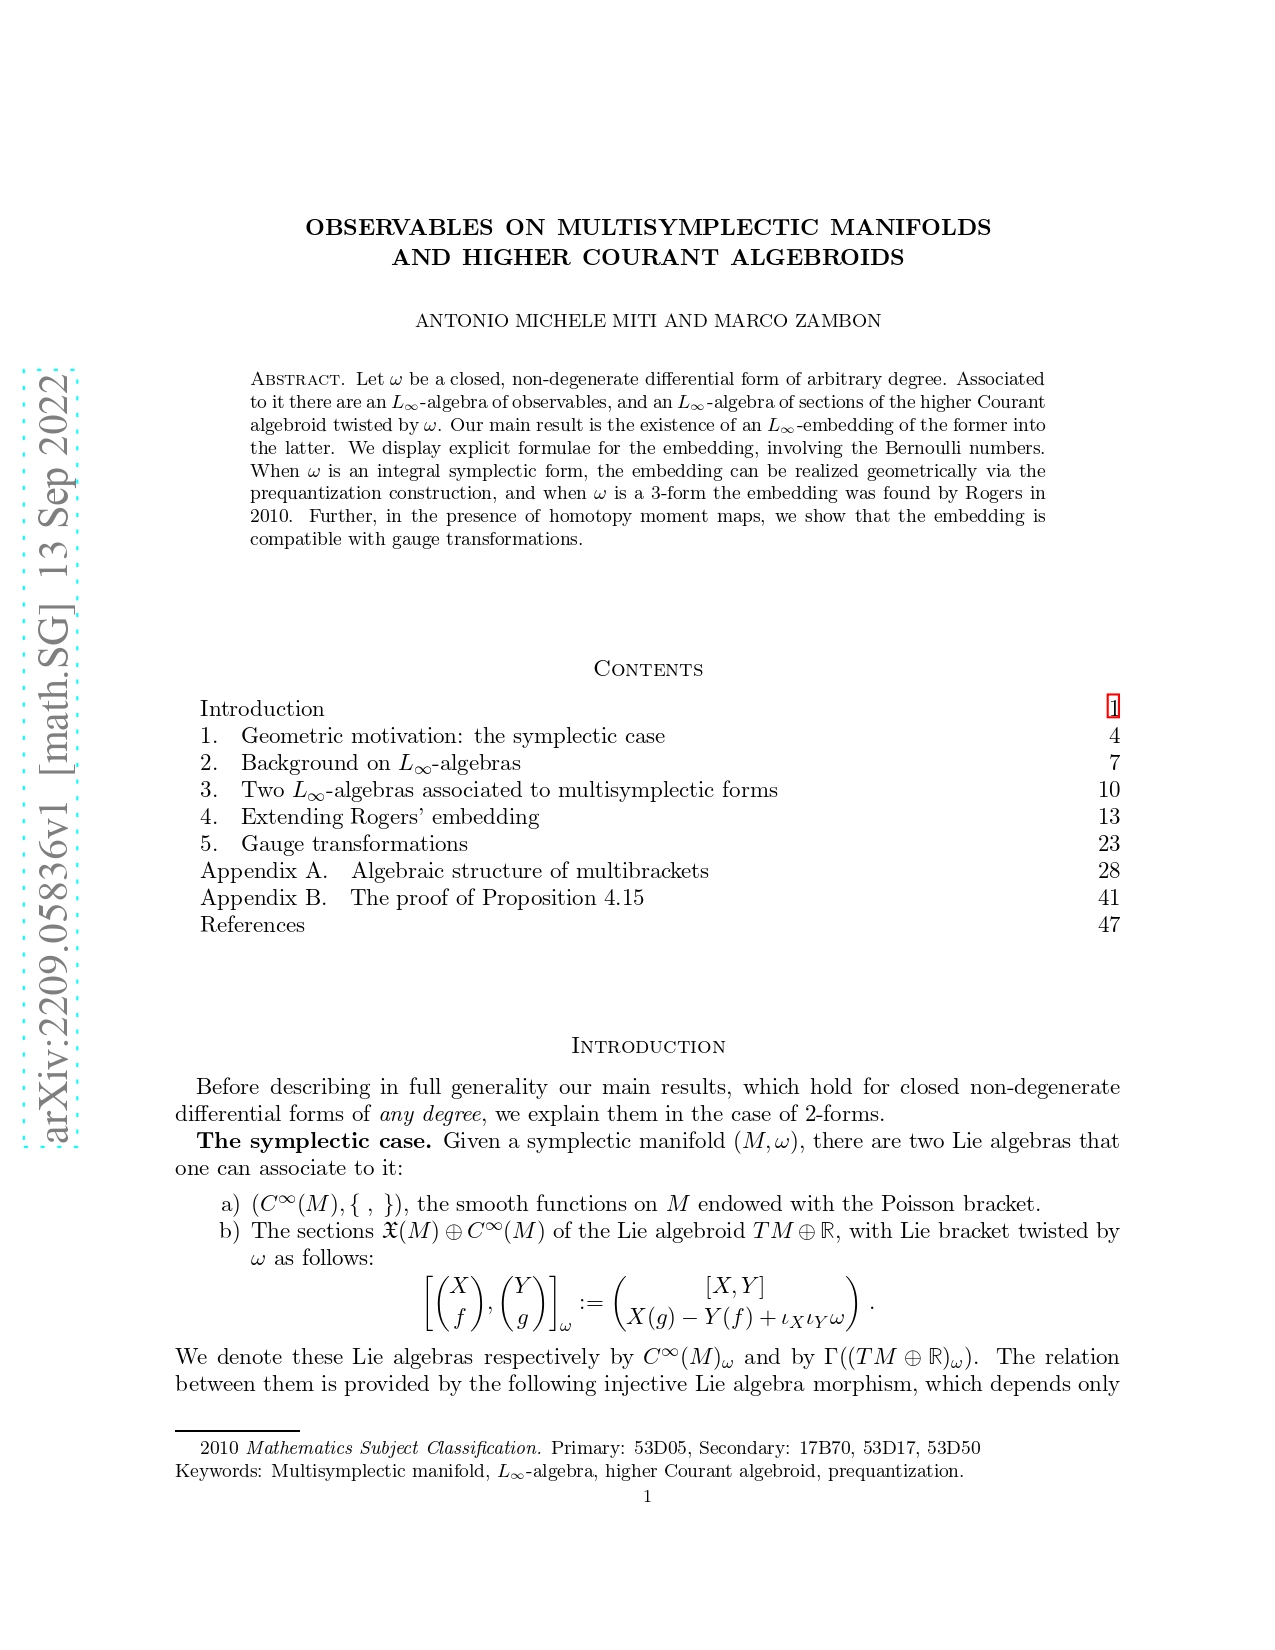
\includegraphics[width=.4\textwidth]{Pictures/arxiv-cover}}
	\end{frame}







%------------------------------------------------------------------------------------------------
% APPENDIX
%------------------------------------------------------------------------------------------------
\appendix



%-------------------------------------------------------------------------------------------------------------------------------------------------
\section{Appendix}
%------------------------------------------------------------------------------------------------

%-------------------------------------------------------------------------------------------------------------------------------------------------
\begin{frame}[fragile]{Homotopy comomentum maps}
	Consider a Lie algebra action $v:\mathfrak{g} \to \mathfrak{X}(M)$  \underline{preserving the $n$-plectic form $\omega$}.
	\vfill
	\begin{defblock}[Homotopy comomentum map \emph{(Callies, Fregier, Rogers, Zambon)} \cite{Callies2016}]
			\includestandalone{Pictures/Frame_Lifting}
	\end{defblock}
	\onslide<4->{
	\begin{lemblock}[HCMM unfolded  \cite{Callies2016}]
			%
			HCMM is a sequence of (graded-skew) multilinear maps:
			\begin{displaymath}
				(f)  = \big\lbrace f_k: \; \Lambda^k{\mathfrak g} \to L^{1-k} \subseteq \Omega^{n-k}(M) 
				~\big\vert~ 0\leq k \leq n+1  \big\rbrace
			\end{displaymath}
			\emph{fulfilling:}%\emph{such that:}
			\begin{itemize}
				\item<5-> $f_0 = 0 $, $f_{n+1} = 0$
				\item<6-> $d f_k (p) = f_{k-1} (
				\tikz[baseline,remember picture]{\node[rounded corners,
                        fill=green!5,draw=green!30,anchor=base]            
            			(target) {$\partial $ };
            	}				
				p)  - (-1)^{\frac{k(k+1)}{2}} \iota(v_p) \omega 
				\qquad\scriptstyle \forall p \in \Lambda^k(\mathfrak{g}),\; \forall k=1,\dots n+1$
			\end{itemize}
		\onslide<7->{
			\tikz[overlay,remember picture]
			{
				\node[rounded corners,
	                 draw=green!30,anchor=base]            
	            	 (base) at ($(current page.east)-(3,3)$) [rotate=-0,align=center] {\footnotesize{\hyperlink{frame:CE-complex}{\emph{Chevalley-Eilenberg boundary op.}}}};
			}	
		\begin{tikzpicture}[overlay,remember picture]
	    	\path[->] (base.west) edge[bend right,green](target.north east);
	    \end{tikzpicture}
	    }
	\end{lemblock}	
	}
	\vfill
\end{frame}
%-------------------------------------------------------------------------------------------------------------------------------------------------




%---------------------------------------------------------------------------------------------------------------------------------------------------
\subsection{Leibniz-algebra of Observables}
\begin{frame}[fragile,t]{Leibniz-algebra of Observables}

	\begin{defblock}[Leibniz algebra of observables]
		\hspace{.25em} $Leib(M,\omega)$ is given by:
		\begin{itemize}
			\item[•] the vector space $$\Omega_{ham}^{n-1}(M,\omega)$$
			\item[•] with the binary bracket 
			\begin{center}
				\includestandalone{Pictures/Equation_Leibbracket}	
			\end{center}
		\end{itemize}	
	\end{defblock}
	\vfill
	\pause
	%
	\begin{propblock}
		\begin{itemize}
			\setlength\itemsep{1em}
			\item[i.] $\vHam_{\llbracket \alpha, \beta \rrbracket} = [\vHam_\alpha,\vHam_\beta]$
			\item[ii.] $\llbracket \sigma, \llbracket \alpha, \beta \rrbracket \rrbracket =
			\llbracket\llbracket \sigma, \alpha \rrbracket, \beta \rrbracket
			+
			\llbracket \alpha, \llbracket \sigma, \beta \rrbracket \rrbracket$
			\item[iii.] $\llbracket \alpha, \beta \rrbracket + \llbracket \beta,\alpha \rrbracket = d \left( \iota_{\vHam_\alpha} \beta + \iota_{\vHam_\beta} \alpha\right)$
		\end{itemize}
	\end{propblock}

\end{frame}
\note[itemize]{
	\item in addition to being extendable to an $L_\infty$-algebra, the space $\Omega^{n-1}_{ham}(M)$ also carries the structure of a Leibniz algebra. This structure is very important for multisymplectic reduction procedures.
	\item 
	\item Take away: Two brackets on $\Omega_H^{k-1}(M)$, ${\color{red}\llbracket\alpha,\beta\rrbracket = \mathcal{L}_{X_\alpha} \beta}$ and ${\color{green}\{\alpha,\beta\}=\iota_{X_\alpha}\d\beta}$,
	Equal up to a coboundary: ${\color{red}\mathcal{L}_{X_\alpha}\beta} = {\color{green}\iota_{X_\alpha}\d\beta} + \d\hspace{1pt}\iota_{X_\alpha}\beta$
}
%---------------------------------------------------------------------------------------------------------------------------------------------------

%-------------------------------------------------------------------------------------------------------------------------------------------------
\begin{frame}[t]{From Symplectic to MultiSymplectic (mechanical perspective)}
	\begin{block}{Historical motivation}
		Mechanics: geometrical foundations of \textit{(first-order)} field theories.
		\begin{itemize}
		 \item[•] Kijowski, W. Tulczyjew \cite{Kijowski1979}; %(1979)
		 \item[•] Cariñena, Crampin, Ibort \cite{Carinena1991b};% (1991)
		 \item[•] Gotay, Isenberg, Marsden, Montgomery \cite{Gimmsy1};%(1998)
		 \\ $\cdots$
		\end{itemize}
	\end{block}
	\vfill
	\pause
	\tcbset{colback=white,
		colbacktitle=white,
		colframe=red!70!black,
		boxrule=1pt,
		colupper=red!70!black,
		arc=15pt}
	\begin{tcolorbox}[enhanced,frame hidden,borderline={0.5pt}{0pt}{red,dashed}]
		\color{red}
		\begin{columns}[T]
			\begin{column}{.20\linewidth}
				\begin{center}
					\huge
					\faWarning
				\end{center}
			\end{column}			
			\begin{column}{.60\linewidth}
				\vspace{-.4em}
				\begin{center}
					The lack of a satisfactory notion of observables hindered the spread of this formalism.
				\end{center}
			\end{column}			
			\begin{column}{.20\linewidth}
				\begin{center}
					\huge
					\faWarning
				\end{center}
			\end{column}			
		\end{columns}
	\end{tcolorbox}
	\vfill
	\pause
	\begin{tcolorbox}[enhanced,frame hidden,borderline={0.5pt}{0pt}{blue,dashed}]
		\color{blue}
		\begin{columns}[T]
			\begin{column}{.20\linewidth}
				\begin{center}
					\huge
					\faQuestionCircle
				\end{center}
			\end{column}			
			\begin{column}{.60\linewidth}
				\begin{center}
					\vspace{-.4em}
					{Why observables are so crucial?\qquad \qquad Quantization!}	
				\end{center}
			\end{column}			
			\begin{column}{.20\linewidth}
				\begin{center}
					\huge
					\faQuestionCircle
				\end{center}
			\end{column}			
		\end{columns}
	\end{tcolorbox}




\end{frame}
\note[itemize]{
	\item Historically, the interest in multisymplectic manifolds, has been motivated by the need for understanding the geometrical foundations of first-order classical field theories.
	The key point is that, just as one can associate a symplectic manifold to an ordinary classical mechanical system (e.g. a single
point-like particle constrained to some manifold), it is possible to associate a multisymplectic
manifold to any classical field system (e.g. a continuous medium like a filament or a fluid). See frame Extra-\ref{Frame:Ms-Field-Mechanics} 
	\item Forger and Romero say: \emph{"The multisymplectic formalism is manifestly consistent with the basic principles of field theory, preserving full covariance, and it is mathematically rigorous because it uses well established methods from calculus on finite-dimensional manifolds. On the other hand, it does not seem to permit any obvious definition of the Poisson bracket between observables. Even the question of what mathematical objects should represent physical observables is not totally clear and has in fact been the subject of much debate in the literature. Moreover, the introduction of n conjugate momenta for each coordinate obscures the usual duality between canonically con- jugate variables (such as momenta and positions), which plays a fundamental role in all known methods of quantization.A definite solution to these problems has yet to be found."}
	
}
%-------------------------------------------------------------------------------------------------------------------------------------------------

%------------------------------------------------------------------------------------------------
\begin{frame}[fragile]{MS geometry and classical field mechanics}\label{Frame:Ms-Field-Mechanics}
		Consider a smooth manifold $Y$,
		\begin{columns}
			\hfill
			\begin{column}{.5\linewidth}
				\emph{Multicotangent bundle} $\bigwedge = \bigwedge^n T^\ast Y$\\
				is naturally $n$-plectic
			\end{column}
			\begin{column}{.4\linewidth}
				\[
				\begin{tikzcd}
					\Lambda \ar[d,"\pi"'] & T \Lambda \ar[d,"T \pi"] \ar[l] \\
					Y								& T Y \ar[l]
				\end{tikzcd}	
				\]
			\end{column}
		\end{columns}
	\pause
	\begin{defblock}[Tautological $n$-form]
		$\theta \in \Omega^n(\Lambda)$ such that:
		\begin{displaymath}
		\begin{split}
			\left[ \iota_{u_1 \wedge \ldots \wedge u_n} \theta \right]_\eta 
			&= \iota_{(T \pi)_\ast u_1 \wedge \ldots \wedge (T \pi)_\ast u_n} \eta \\
			&= \iota_{u_1 \wedge \ldots \wedge u_n} \pi^\ast \eta 
			\qquad \qquad \forall \eta \in \Lambda \, , \: \forall u_i \in T_\eta \Lambda 		
		\end{split}
		\end{displaymath}
	\end{defblock}
	\vfill
	\begin{columns}
		\begin{column}{.6\linewidth}
			\begin{defblock}[Tautological (multisymplectic) (n+1)-form]
				$$\omega := d \theta$$
			\end{defblock}
		\end{column}
		\begin{column}{.4\linewidth}
		 	\begin{claimblock}$\omega$ is not degenerate.\end{claimblock}	
		\end{column}
	\end{columns}	
	\pause
	\begin{keywordblock}
		\begin{tabular}{|c|c|c|}
			\hline 
			point-particles mechanics & $\rightsquigarrow$ & classical fields mechanics \\
			%(finite discrete DOF) & & (finite dimensional continuous DOF) \\
			\hline 
			symplectic & $\rightsquigarrow$ & multisymplectic \\ 
			\hline 
			Observables (Poisson) algebra & $\rightsquigarrow$ & Observables $L-\infty$ algebra
			 \\ 
			\hline 
			Co-moment map & $\rightsquigarrow$ & Homotopy co-momentum map \\ 
			\hline 
		\end{tabular} 
	\end{keywordblock}

	
\end{frame}
\note[itemize]{
	\item This example is significant from the perspective of geometric classical field theory:
		\begin{displaymath}
			\frac{\text{classical mechanics}}{\text{symplectic geo.}} =
			\frac{\text{classical field mechanics}}{\text{multisymplectic geo.}}
		\end{displaymath}
	\item Multicotangent bundle is the \emph{Higher analogue} of the cotangent bundle.
	(but it is not yet the analogue of a \emph{phase space}.)
\item The multiphase space is the sub-bundle of $n$-forms vanishing when contracted with 2 vertical fields.
  	\item The reason why this sub-bundle has a particular role is that it can be proved to be isomorphic to a suitable dual of the first Jet bundle.
  	\item For further details see Gotay et al. \href{https://arxiv.org/abs/physics/9801019}{arXiv:physics/9801019}. For a pictorial representation of all the structures involved in the geometric mechanics of I order classical field theories see appendix, pag: \ref{frame:Gimmsy}.
}
%------------------------------------------------------------------------------------------------	


%------------------------------------------------------------------------------------------------
% https://en.wikibooks.org/wiki/LaTeX/Bibliographies_with_biblatex_and_biber
\begin{frame}[t,allowframebreaks]{Extended Bibliography}
	\bibliographystyle{alpha}
	\bibliography{bibfile}
\end{frame}
%------------------------------------------------------------------------------------------------









%------------------------------------------------------------------------------------------------
\end{document}

